\chapter{Inspirasjon og tidligere arbeid}
I dette kapittelet vil eksisterende digitale løsninger som brukes i sammenhenger relevant til sporing og registrering av sau undersøkes og vurderes. Avslutningsvis vil arbeidet og resultatet fra fordypningsprosjektet bli presentert, som masteroppgaven har lagt til grunne og bygd videre på.  

\section{Eksisterende løsninger}
I dag finnes det ulike digitale løsninger som forenkler prosessen med tilsynstur på utmarksbeitet. Disse løsningene gjør en av to ting; enten bytter ut dagens system med sporingsbrikker eller et nytt digitalt system for manuell registrering av dyr på utmarksbeite. Slike løsninger skal vi presentere og undersøke i dette kapittelet. 

\subsection{Elektronisk sporing av dyr} \label{sporing}
 Utviklingen av teknologi knyttet til småfehold har utviklet seg raskt de siste ti årene for å gjøre det enklere for bonden å ha kontroll på småfeet på beite \cite[~s.49-50]{BungerSmafenaring2018}. For teknologi brukt utendørs, er automatisk sporing av dyrene med såkalte radiobjeller mest brukt blant bønder \cite[~s.50]{BungerSmafenaring2018}. Slike radiobjeller plasseres rundt halsen på sauen når den er på beite og gir signaler om dyrenes lokasjon til bonden ved hjelp av \acrshort{gps} eller mobilnettet \cite{Fremstad2020SauebnderRuralis}. De største aktørene i det norske markedet for radiobjeller er Telespor \cite{Telespora} og Findmy. De seneste årene har disse aktørene har fått konkurranse fra nye aktører som blant annet Smartbjella \cite{SmartbjellaSporing}.  
 
 \begin{figure}[H]
\centering
\captionsetup{width=.8\linewidth}
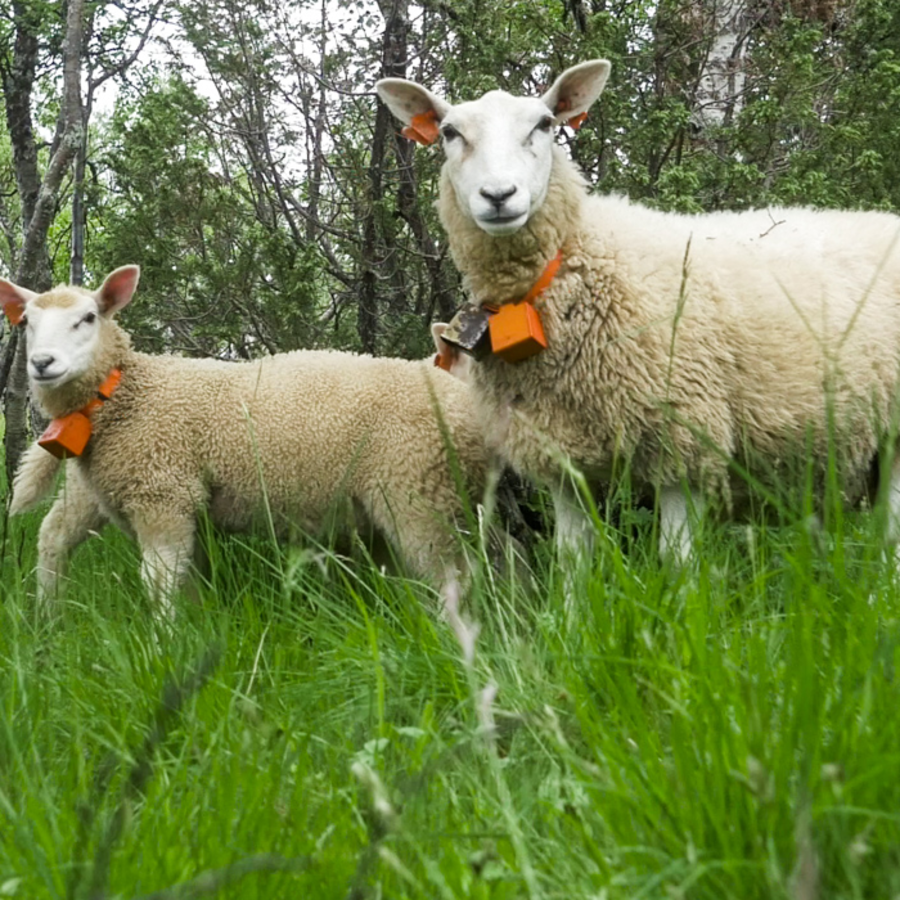
\includegraphics[scale=0.3]{Figurer/Bilder/findmy_bjeller.png}
\caption{Sauer utstyrt med radiobjeller fra FindMy}
\source{\cite{findmyProdukt}}
\label{fig:radiobjeller}
\end{figure}
 
 \subsubsection{Telespor}
 Telespor har vært på markedet siden 2004 med elektronisk sporing av husdyr på beite over lengre tid med "Radiobjella" som benytter seg av GPS lokalisering, og har lansert sin fjerde generasjons radiobjelle \cite[~s.69]{kvamRoleAdvisoryServices2019} \cite{ProduktTelespor}. Tidligere generasjoner av radiobjella brukte \acrshort{gsm}/\acrshort{gprs}, det vil si 2G mobilnettet, for å motta GPS posisjon fra satellitter til Telespors server som deretter videresendte informasjonen til kundens brukerportal  \cite{Telesporsystemet}. Dagens fjerde generasjons radiobjelle benytter seg av nyere \acrfull{nbiot} og \acrshort{lte}, som muliggjør at sensorer og andre enheter kan kommunisere med 4G-nettet raskere og med svært lav energibruk \cite{lorentzenTingenesInternettInntar2018, ProduktTelespor}. Telespor bruker Telenors IoT-dekning på 4G-nettet. Dette gjør at radiobjellene er avhengig av at det er dekning i området for å kunne kommunisere med bonden. Radiobjellene er også utstyr med bevegelsessensorer som kan utløse tre alarmer \cite{ProduktTelespor} dersom: 
 \begin{itemize}
     \item Dyret har ikke beveget seg de siste 3 timene.
     \item Dyret har vært på samme posisjon i en lengre periode.
     \item Radiobjella har ikke klart å sende sin posisjon de siste 2 rapportene
 \end{itemize}
 \noindent
Sendeintervall og alarmsensitivitet kan endres på når som helst av brukeren \cite{ProduktTelespor}. Selve bjellene er utstyrt med utskiftbare batteri som det anbefales at man skifter etter hver sesong \cite{ProduktTelespor}. Telespor bruker en betalingsmodell der brukere må betale en sum for radiobjellene og et sesongbasert abonnement som dekker både mobildatatrafikken, tilgang til brukerportalen og et batteri \cite{telenorDekningIoTPa, TelesporNettbutikka}. Per dags dato er prisen på en fjerde generasjons radiobjelle 1124 kr og sesongabonnement 124 kr \cite{TelesporNettbutikka}.

\subsubsection{FindMy}
FindMy, tidligere kalt FindMySheep, ble skapt av sauebønder i 2009 som ønsket elektronisk sporingsutstyr som ikke var avhengig av mobilnettet \cite{findmyOmOss}. FindMys e-bjeller er bygd rundt lavbane satellitt teknologi og er dermed ikke avhengig av verken \acrshort{gsm} eller \acrshort{nbiot} for å fungere og vil i praksis fungere over hele verden \cite{findmySatelitt}. Det vil si at e-bjella har dekning så lenge den har fri sikt til himmelen. E-bjella har også en funksjon der den vil prøve å sende signaler flere ganger for å få tilfredstillende resultat dersom e-bjella er i et område med utfordrende terreng og topografi \cite{findmyDekningHeleNorge}. Alle e-bjellene kan settes opp med egendefinerte meldingsplaner som bestemmer hvor ofte man får oppdateringer om dyrets posisjon i løpet av en dag \cite{findmySlikFungererSatellittene}. I tillegg til elektronisk sporing har e-bjella Model 2 funksjoner som sporingsdata og tilvekstkart fra Sauekontrollen, søk med Bluetooth, geofencing, urovarsel som detekterer unormal adferd i flokken og sporlogg som samler posisjoner e-bjella har sendt i en valgt periode for å gi innsikt beitemønster \cite{findmyFunksjoner}. FindMy anbefaler selv at man sporer minst 25\% av dyreflokken for å få god oversikt over dyrene \cite{findmyProdukt}. Ca. 40 000 e-bjeller fra FindMy er i bruk per dags dato \cite{findmyFunksjoner}. Per i dag koster én enkelt e-bjelle 1849 kr, og årlig brukeravgift kommer på 229 kr per bjelle \cite{findmyShop}. Lik som Telespor har også e-bjella til FindMy utskiftbarebatteri, men disse skal vare 2-3 beitesesonger og koster 99 kr per stykk \cite{findmyBrukeravgift}. 

\subsubsection{Smartbjella}
Smartbjella/Smartbells ble lansert i 2019 etter at ansatte ved morselskapet StalkIT \cite{HomeStalkITNo} oppdaget at deres teknologi for å spore opp konteinere kunne være nyttig for å spore sauer på beite \cite{SMARTBELLSEmisjonskampanjeFolkeinvest2019}. Smartbjella var den første aktøren som benyttet seg av IoT-teknologi innenfor dyresporing, etter å ha inngått avtaler med Telenor og Telia om å bruke deres \acrshort{nbiot} nettverk  \cite{henriksenKonkurransenBeitetechHardner2020}. Det benyttes også \acrshort{gnss} for nøyaktig posisjonering \cite{PRODUKTSmartbjellaSporing}.  Smartbjella nyeste versjon 2 som er ute for pre-salg i 2021 inkluderer dødsalarm, frekvensstyring av signalene fra bjellen, historisk bevegelsesmønster, temperaturmåler, Bluetooth og mulighet til å sette opp geofence \cite{PRODUKTSmartbjellaSporing}. Smartbjella skal være vedlikeholdfri per sesong \cite{PRODUKTSmartbjellaSporing}. Ved normale værforhold og med et rapporteringsintervall på 24 timer skal batteriet i Smartbjella holde opptil 15 år. \cite{PRODUKTSmartbjellaSporing}. Prisen for Smartbjella 2 ligger på 949 kr per enhet og abonnement på en sesongbruk av smartbjella ligger på 100 kr per enhet \cite{SmartbjellaPresalg2021}. Det er også mulig å leie radiobjeller \cite{SMARTBELLSEmisjonskampanjeFolkeinvest2019}. Per dags dato er det 18000 radiobjeller fra Smartbjella i Norge \cite{SmartbjellaSporing}. 

\subsubsection{Konklusjon/Evaluering}
Alle bedriftene som er nevnt i forrige delkapittel er i markedet for elektronisk sporing av dyr på utmarksbeite og arbeider med å gjøre det lettere for bønder å lokalisere dyreflokken og få tilbakemeldinger om dyrenes tilstand. Teknologiene som utnyttes for elektronisk sporing er relativt like, spesielt etter at Telespor også byttet over til å bruke \acrshort{nbiot} og \acrshort{lte}, med unntak av FindMy som benytter seg av lavbane satellitter. Dette er en fordel her i Norge, der dyrene ofte ferdes på øde steder uten mobildekning på utmarksbeite. Alle aktørene tilbyr også en form for alarmfunksjonalitet som gir tilbakemelding dersom et dyr har vært inaktiv over en periode. Betalingsmodellene er også tilnærmet identiske, med en pris for selve radiobjellene og brukeravgift/abonnement på servicetjenester, samt tilleggskostnader for batteri som eventuelt må skiftes ut. Her skiller Smartbjella seg ut ved at batteriene har mye lengre levetid. Smartbjella gir mer fleksibilitet da det er mulig å bare leie bjellene ved behov ønskelig \cite{SMARTBELLSEmisjonskampanjeFolkeinvest2019}. Prismessig ligger Telespor og FindMy på rundt 1500-2000 kr for en hel pakke inkludert bjelle og brukeravgift, mens Smartbjella er rimeligere med enheter og brukeravgift på rundt 1000 kr. 
\newline 
\newline
Store kostnader knyttet til utstyr og vedlikehold er nettopp en av grunnen til at mange bønder tidligere ikke ønsket å benytte seg av radiobjeller, men de siste årene med nyere, mer stabil teknologi og konkurranse fra flere aktører på markedet som presser prisene ned, er det nå flere og flere bønder som prøver ut  radiobjeller. I rovdyrutsatte områder kan også beitelag søke om tilskudd til konfliktdempende tiltak som deriblant elektronisk overvåkningsutstyr, der Statsforvalteren kan dekke deler av kostnadene for slik investering Dette har gjort at flere bønder fikk testet radiobjeller og senere begynt å benytte seg av det \cite[~s.61, 66]{kvamRoleAdvisoryServices2019} \cite{landbruksdirektoratetTilskuddTilTiltak}.  
\newline
\newline
I 2009 - 2012 ble det utført et nasjonalt beiteprosjekt på vegne av Statens landbruksforvaltning (nå Landsbruksdirektoratet) med formål å få bedre sauehold med mindre tap av dyr på beite \cite{statenslandbruksforvaltningNasjonaltBeiteprosjekt20092013}. Utprøvingen av  radiobjeller ble evaluert av \acrfull{tfou} \cite[~s.8]{statenslandbruksforvaltningNasjonaltBeiteprosjekt20092013}. Rapporten konkluderte med at det antakelig er en forebyggende tapsreduserende effekt med bruk av radiobjeller og at det førte til bedre dyrevelferd ettersom bjellene ga raskere avdekking av unormal adferd blant dyrene samt mer effektiv sanking på høsten \cite[~s.40]{statenslandbruksforvaltningNasjonaltBeiteprosjekt20092013}. Bøndene selv rapporterte økt produktivitet fordi radiobjellene gjorde arbeidet om å lokalisere dyrene i sammenheng med tilsyn og sanking lettere, som igjen førte til høyere tilfredshet blant bøndene og økt motivasjon til å bruke utmarksbeite \cite[~s.41]{statenslandbruksforvaltningNasjonaltBeiteprosjekt20092013}, \cite[~s.60]{kvamRoleAdvisoryServices2019}. Tapte dyr med radiobjeller hadde økt gjenfinningsrate og bedre mulighet til å fastslå dødsårsak enn dyr uten radiobjeller \cite[~s.40]{statenslandbruksforvaltningNasjonaltBeiteprosjekt20092013}. 
\newline
\newline
Selv om overvåkningsteknologien for dyr på utmarksbeite stadig forbedres og prisen for utstyret senkes, er det fortsatt ikke vanlig å sette radiobjeller på alle dyrene. Elektronisk sporing av dyr erstatter ikke oppsynsturer som bøndene fortstatt er lovpålagt å dra til beitet for å sjekke dyrenes tilstand, men det er et nyttig verktøy som gjør dette arbeidet lettere å gjennomføre.

\subsection{Registrering av dyr i utmark} 
Per dags dato er det ingen aktive applikasjoner som legger til rette for registrering av dyr i utmark, men det finnes løsninger som har vært innom denne ideen tidligere. Beitesnap var en applikasjon som tok for seg registrering av tilsyn for husdyr på beite, både for bønder under beitesesongen og for privatpersoner som ønsker å melde fra om beitedyrsobservasjoner \cite{BeitesnapRevolusjonerendeVerktoy}. I tillegg er det gjennomført tidligere masteroppgaver med lignende problemstilling, som for eksempel applikasjonen Lambo som ble utviklet for oppgaven \textit{Effektivisering av manuell oppfølging av sau på utmarksbeite} fra 2018 \cite{dystheEffektiviseringAvManuell2018}. Det er også flere pågående masteroppgaver per våren 2021 som utforsker samme tema som denne masteroppgaven.  

\subsubsection{Beitesnap}
Beitesnap av Fant AS er en applikasjon som ble lansert i 2017 som et verktøy for å registrere observasjoner av husdyr på beite \cite{BeitesnapRevolusjonerendeVerktoy}. Applikasjonen avsluttet driften fra og med 2020 grunnet dårlig økonomi som følge av få brukere \cite{BeiteSnapFacebook2020}. Applikasjonens målgrupper var beitebrukere som kunne legge inn sitt beiteområde og dyrenes individnummer slik at de kan få meldinger fra andre som observerer skadde eller døde dyr innenfor bondens beiteområde \cite{BeitesnapRevolusjonerendeVerktoy}. Alle registreringene fra beitesesongen ble samlet og utformet til en rapport som kunne sendes inn til myndighetene \cite{BeitesnapRevolusjonerendeVerktoy}. Beitesnap var også koblet opp mot Norgeskart \cite{NorgeskartKartverketNo}, slik at det var mulig å spore oppsynsturene med \acrshort{gps} \cite{BeiteSnapFacebook2020}. Kartet kunne lastes ned på forhånd for offline bruk \cite{BeitesnapRevolusjonerendeVerktoy}. For å få tilgang til en Beitebruker-konto på Beitesnap, var det en årlig avgift på 1200 kr + MVA \cite{BeitesnapRevolusjonerendeVerktoy}. Privatpersoner som ønsket å sende inn sine observasjonen kunne opprette en gratis bruker, som hadde mulighet til å sende inn bilder med informasjon om dyr de møter på i utmarka \cite{BeitesnapRevolusjonerendeVerktoy}. Dersom observasjonen er innenfor et registrert beiteområdet, vil den aktuelle bonden få beskjed om det \cite{BeitesnapRevolusjonerendeVerktoy}. 
\newline
\newline
Beitesnap har mye lik funksjonalitet som Sauron, men hvordan informasjonen registreres er nokså ulik. I Beitesnap registreres et bilde av observasjonen, hvilket dyreslag som er registrert, om dyret var sett, skadd eller dødt og eventuelt individnummeret til dyret \cite{beitesnapKomplettBrukermanualBeitebrukere2017}. All annen informasjon, som totalt antall dyr, antall søyer og lam, farge på dyrene, øremerker eller bjelleslips må dermed skrives i fritekst. Å observere dyrene på lang avstand for å så måtte taste inn all informasjonen kan være utfordrende, samtidig som det gjør at innrapporteringene er mindre strukturerte. (Prisen for å ha en beitebruker-konto virker også nokså stiv for sauebønder som allerede betaler mye penger for å bruk av elektronisk sporingsutstyr). 

\begin{figure}[H]
\centering
\captionsetup{width=.8\linewidth}
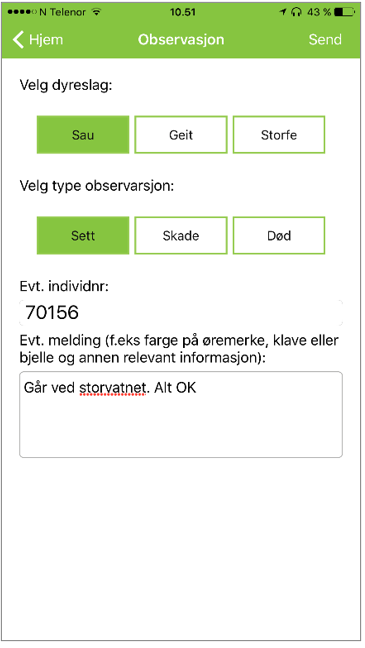
\includegraphics[scale=0.7]{Figurer/Bilder/beitesnap.png}
\caption{Skjermbilde av Beitesnaps registreringsside}
\source{\cite{beitesnapKomplettBrukermanualBeitebrukere2017}}
\label{fig:beitesnap}
\end{figure}

\subsubsection{Tidligere og pågående masteroppgaver}
Det er flere gjennomførte og pågående masteroppgaver fra NTNU som har arbeidet med å effektivisere oppsyn av sauer på utmarksbeite. Denne masteroppgaven har tatt inspirasjon fra masteroppgaven \textit{Effektivisering av manuell oppfølging av sau på utmarksbeite} \cite{dystheEffektiviseringAvManuell2018} skrevet av Stian Dysthe og Andreas Kjerstad der professor Hvasshovd også var veileder. Deres mål for prosjektet var:
\newline
\newline
\textit{Utvikle et produkt som gjør det lett og effektivt å registrere detaljert, strukturert, lokasjonsbasert informasjon om sau på beite, samtidig som det møter behovet til bøndene og krav fra myndighetene} \cite[~s.13]{dystheEffektiviseringAvManuell2018}.
\newline
\newline
I den sammenhengen utviklet de applikasjonen Lambo, som har en del fellestrekk med både Beitesnap og Sauron. Lambo har funksjonalitet som online og offline kart med GPS-sporing av brukerens rute og registrering av observasjoner av både husdyr og rovdyr \cite{dystheEffektiviseringAvManuell2018}. I motsetning til Beitesnap, har Lambo en mer detaljert innrapportering av observasjoner, der brukeren må gå gjennom et registreringsskjema som brukeren må trykke gjennom for å registrere en observasjon istedetfor å skrive det inn som fritekst. Brukeren vil først bli spurt om observasjonen gjelder sau, skadet sau, død sau, ullfunn, hund, rovdyr, reinsdyr eller annet, og deretter få spørsmål om relevante underkategorier som antall, farge osv \cite[~s.84-85]{dystheEffektiviseringAvManuell2018}. Måten å registrere informasjon er det som vil skille Sauron fra Lambo, ettersom denne masteroppgaven vil ha et særskilt fokus på hvordan å registrere observasjonene uten å se på mobilskjermen.

\begin{figure}[H]
\centering
\captionsetup{width=.8\linewidth}
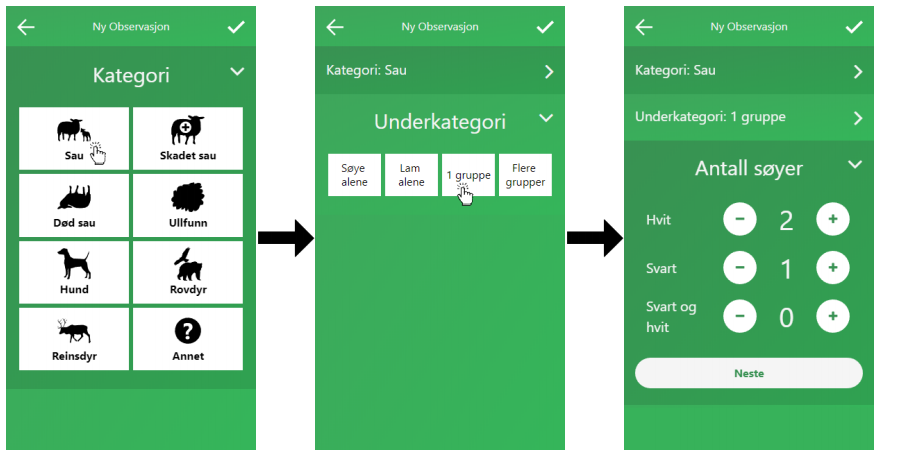
\includegraphics[scale=0.5]{Figurer/Bilder/lambo.png}
\caption{Skjermbilde fra Lambos registreringsskjema}
\source{\cite{dystheEffektiviseringAvManuell2018}}
\label{fig:lambo}
\end{figure}
 
\section{Fordypningsprosjekt}
Denne masteroppgaven bygger videre på arbeidet gjort under fordypningsprosjektet "Tilsyn med Sau På Beite" \cite{Abtahi2020TilsynBeite} som ble gjennomført høsten 2021. Mens denne masteroppgaven går ut på å utvikle et helhetlig produkt for å bistå gjetere på oppsynstur, fokuserte fordypningsprosjektet spesifikt på selve registreringen av sau. Målet med fordypningsprosjektet var: 
\newline
\newline
\textit{Designe og utvikle en applikasjon som muliggjør effektiv registrering av sauer på utmarksbeite i situasjoner der brukeren kontinuerlig benytter seg av kikkert og dermed ikke kan se på skjermen.} \cite[~s. 3]{Abtahi2020TilsynBeite}
\newline
\newline
Denne problemstillingen ble løst ved å først undersøke brukergrensesnitt for skjermer som var utviklet med tanke på bruk i blinde. Det ble så valgt tre ulike brukergrensesnitt, en med Sveiping, en med knapper og en med en kombinasjon av de tidligere to grensesnittene som det ble utviklet prototyper for. Alle brukergrensesnittene benyttet seg av tekst-til-tale for å gi informasjon om registreringen til brukeren mens registreringen pågikk. Deretter ble det utformet og gjennomført ni brukertester som undersøkte feilraten ved registrering, effektiviteten ved kortest gjennomføringstid og hva som var den beste måten å gi tilbakemelding på når skjermen var utilgjengelig. Både de kvantitative og kvalitative resultatene fra brukertestene tilsa at grensesnittet som benyttet seg av Sveiping fungerte best for formålet. Dette resultatet har blitt tatt videre i masteroppgaven, og det er begrunnelsen for at det blir brukt en kombinasjon av sveiping og tapping i brukergrensesnittet for registrering av sau i Sauron.

\section{Konklusjon}
Det brukes stadig mer og mer digital teknologi for å assistere bønder i deres arbeid med å slippe dyr på utmarksbeite. Et av de mer brukte digitale verktøyene som bistår i oppsynsturer er digitale sporingsutstyr som radiobjeller som settes på dyrene og sporer deres lokasjon med GPS-teknologi eller \cite{nbiot}. Per i dag er det minst 3 aktører i Norge som driver radiobjeller; Telespor, FindMy og Smartbjella. Disse aktørene benytter seg av GPS-teknologi som enten \acrshort{nbiot}-nettet eller lavbane satellitt teknologi for sporing, og har i tillegg andre funksjoner som blant annet dødsalarm, tilpasning av innrapportering og geofencing. Tidligere prosjekter som har evaluert bruken av elektronisk overvåkning av dyr på utmarkbeite har konkludert med at radiobjellene kan forebygge tap på beitet ved at farlige situasjoner raskere blir avdekket og samtidig fører til mer effektiv sanking av dyrene på høsten. Likevel vil ikke radiobjeller erstatte manuelle oppsynsturer med det første ettersom norske myndigheter krevet at oppsynsturer skal bli utført ukentlig. Applikasjoner som Beitesnap og Lambo, som ble også utviklet i en masteroppgave, har blitt brukt som inspirasjon. Det ble konkludert at disse applikasjonene manglet funksjonalitet som muliggjør registrering av sau uten å se på mobilskjermen. Hvordan å utføre handlinger på best mulig måte uten å se på skjermen ble undersøkt i fordypningsprosjektet. Under fordypningsprosjektet ble det utformet tre ulike brukergrensesnitt som deretter ble brukertestet. Resultatene fra testene viste at en kombinasjon av sveiping og tapping fungerte best for registrering av sau og dette brukergrensesnittet er brukt som utgangspunkt i masteroppgaven. 